\documentclass[conference]{IEEEtran}
\IEEEoverridecommandlockouts
% The preceding line is only needed to identify funding in the first footnote. If that is unneeded, please comment it out.
\usepackage{cite}
\usepackage{amsmath,amssymb,amsfonts}
\usepackage{algorithmic}
\usepackage[hidelinks]{hyperref}
\usepackage[noabbrev,capitalize]{cleveref}
\usepackage{array, booktabs, makecell}
\usepackage{graphicx}
\usepackage{textcomp}
\usepackage{xcolor}
\usepackage{caption}
\usepackage{subcaption}
\newcommand\norm[1]{\left\lVert#1\right\rVert}
\def\BibTeX{{\rm B\kern-.05em{\sc i\kern-.025em b}\kern-.08em
    T\kern-.1667em\lower.7ex\hbox{E}\kern-.125emX}}
\newcommand{\red}[1]{\textcolor{red}{#1}}

\graphicspath{../}
\hypersetup{
    colorlinks=true,
    linkcolor=black,
    filecolor=black,      
    citecolor=black,
    urlcolor=blue,
    pdfpagemode=FullScreen,
    }

\begin{document}

\title{An Indirect, Multiscale and Robust Approach to Global Motion Estimation}

\author{\IEEEauthorblockN{Filippo Daniotti}
\IEEEauthorblockA{\textit{DISI, University of Trento} \\
Trento, Italy\\
filippo.daniotti@studenti.unitn.it\\
232087}
\and
\IEEEauthorblockN{Samuele Conti}
\IEEEauthorblockA{\textit{DISI, University of Trento} \\
Trento, Italy\\
samuele.conti@studenti.unitn.it\\
229294}
}

\maketitle

% add page number
\thispagestyle{plain}
\pagestyle{plain}

\begin{abstract}
The problem of global motion estimation (GME) deals with the separation, in a video sequence, of two different types of motion: the \emph{egomotion} of the camera recording the video, and the actual motion of the objects recorded. The literature presents a number of possible approaches to the GME problem; here, we aim to combine some of the most effective strategies to compute the motion of the camera. We adopt an indirect approach based on a perspective motion model (as \cite{Dufeaux2000}). Following a multi-resolution approach, at the lower-resolution level, we use block matching estimation to get a dense motion field; then, at each following (higher-resolution) level we optimize the current parameters of the motion model with gradient descent. During the process of gradient descent the outliers are discarded, in order to get a robust estimation. The final result consists in the optimized list of parameters of the motion model.  
\end{abstract}

\begin{IEEEkeywords}
multi-resolution, robust, indirect, global motion estimation, computer vision, video processing
\end{IEEEkeywords}

\section{Introduction}
\label{sec:01-intro}
The problem of global motion estimation (GME) deals with the separation, in a video sequence, of two different types of motion: the egomotion of the camera recording the video, and the actual motion of the objects recorded. This task is crucial for a number of application, for instance:
\begin{itemize}
    \item removal of camera shaking or noisy motion;
    \item study of the motion of the camera itself;
    \item object segmentation and recognition;
    \item object tracking.
\end{itemize}

For these reasons, motion estimation is a task that has long been studied, hence in the literature we can find a variety of approaches to the problem. In this work we concentrated on some of the most effective approaches and combined them to get an indirect, multi-resolution and robust approach to GME.

The document is structured as follows: in Sec.\ref{sec:02-gme} we sum up the fundamental aspects of the GME problem and the standard approaches to solve these problems. In Sec.\ref{sec:03-implementation} we discuss the strategies we chose for our implementation, and in Sec.\ref{sec:04-results} we present the results of this work. The conclusions in Sec.\ref{sec:conclusions} sum up the work and draw a path for future development.

\section{Global Motion Estimation}
\label{sec:02-gme}
Videos are, at their core, sequences of images called frames; we can spot the motion happening between a given pair of frames by detecting which pixels changed position with respect to that pair of frames.

This information can be encoded in a human-understandable format by presenting the \textit{needle diagram} of the two frames; this kind of representation is shown in \cref{fig:needle-diagram}.

\begin{figure}
    \centering
    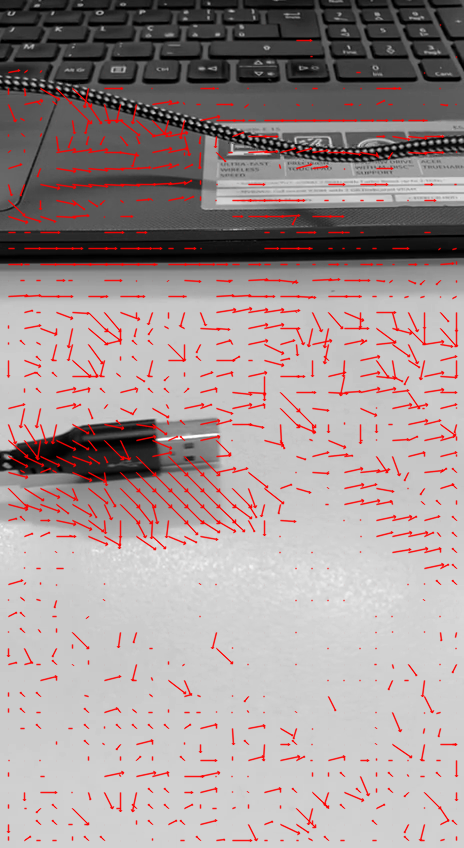
\includegraphics[width=.7\linewidth]{../assets/images/bbme-0-res.png}
    \caption{Needle diagram between two frames of a video sequence.}
    \label{fig:needle-diagram}
\end{figure}

It is pretty clear what information this figure is conveying: for each couple of frames we mark with an arrow the shift that the pixel has made. This gives us an indication of the actual movement of the recorded objects.

However, the motion that we are able to extract from the two frames is what is usually called "apparent motion", which is a combination of two different factors:
\begin{itemize}
    \item the global motion, which corresponds to the motion of the camera;
    \item the effective motion of the objects recorded.
\end{itemize}

An important task in computer vision is the global motion estimation, which aims to distinguish these two different types of motion.
In particular, this information is highly important for a number of applications, amongst which we find video coding, motion compensation, object segmentation and egomotion estimation.

The task of distinguishing which movement is to be classified as global motion and which one is to be classified as object motion instead is not so easy. In fact, there is no clear feature that distinguishes the moving objects from the static background, and this leads to the need for complex tools to differentiate the two types of motion.

% Therefore, to model motion we usually assign to each pixel a vector which describes the shift in the coordinates of that pixel. 

\subsection{Motion Models}
\label{sec:motion-models}

The main approach to global motion estimation consists in using a motion model to describe the motion of the camera.

% What is a motion model?
Motion models describe the motion of the entire visual field through an equation. Basically, the underpinning idea is to write an equation which, given a pixel in a certain position $(x,y)$, returns the position that the same pixel will have in the next frame, if its motion is due only to camera motion.

There is a number of motion models that can be used to describe global motion, ranging from very simple translational models - that can describe only translation motion - to more complex models, allowing to describe pan, tilt, zoom and roll motion patterns. The reader can use as reference \cref{fig:camera-motion} as an illustration of these types of motion.

\begin{figure}
    \centering
    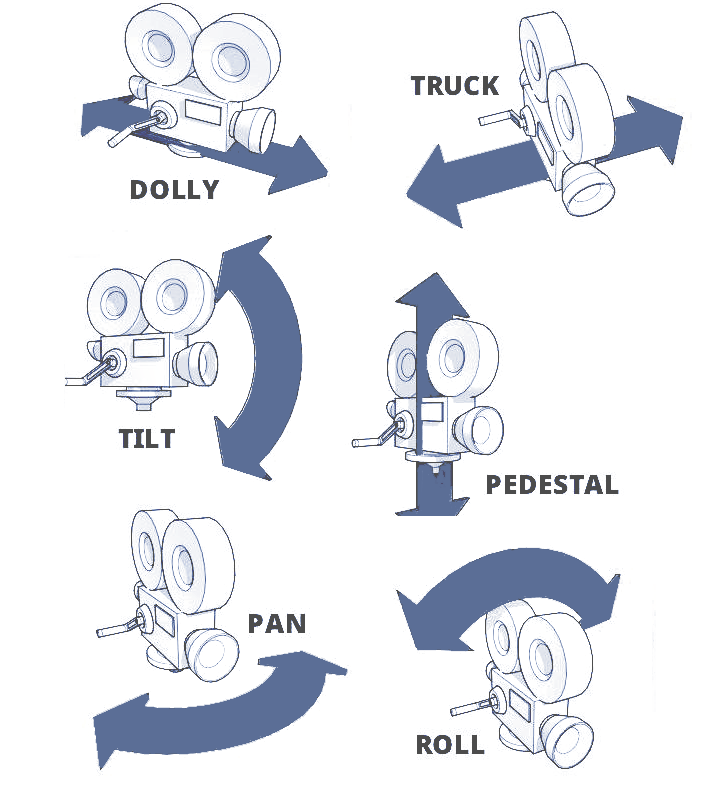
\includegraphics[width=.7\linewidth]{../assets/images/camera-movement.png}
    \caption{Different types of camera motion. Source: \url{https://cinestudy.org/2020/06/29/camera-movement/}.}
    \label{fig:camera-motion}
\end{figure}

All the motion models are defined as functions of some parameters; to get the camera motion in a certain sequence we need to estimate the parameters of the motion model for that precise sequence. Taking as example the motion model we used in this project - the affine motion model - the shift in the position of a pixel can be described as in \cref{eq:affine-model-representation}.

\begin{equation}
    \label{eq:affine-model-representation}
    p' = 
    \begin{bmatrix}
        X' \\ Y' \\ Z'
    \end{bmatrix}
    =
    \begin{bmatrix}
        r_1 & r_2 & r_3 \\
        r_4 & r_5 & r_6 \\
        r_7 & r_8 & r_9 
    \end{bmatrix}
    \begin{bmatrix}
        X \\ Y \\ Z
    \end{bmatrix}
    +
    \begin{bmatrix}
        T_X \\ T_Y \\ T_Z
    \end{bmatrix}
    = Rp + T
\end{equation}

Here $p'$ represents the position of the pixel after the camera motion. The matrix $R$ is used to describe rotation and the vector $T$ for the translation component.

The affine motion model can describe
\red{check precisely in the book}

Usually the affine model is used under the assumptions that the rotation and translation are on the image plane, and that depth $Z$ is approximately constant (as from \cite{WangBook}); these assumptions are reasonable as long as the motion occurring between the two frames we are analyzing is not too large.
Under these assumptions, the affine model can be represented as \cref{eq:affine-model-direct-estimation}, where we need to estimate the 6 parameters $a =[a_1, a_2, a_3, b_1, b_2, b_3 ]$.

\begin{equation}
    \label{eq:affine-model-direct-estimation}
    \begin{split}
        \Delta x &= a_1 x_0 + a_2 y_0 + a_3 \\
        \Delta y &= b_1 x_0 + b_2 y_0 + b_3
    \end{split}
\end{equation}

\subsection{Parameter Estimation}
There are two different approaches to estimate the parameters of a motion model:
\begin{itemize}
    \item a direct approach, which computes the best parameters by optimizing an overdetermined system in the pixel domain;
    \item an indirect approach, which minimizes the approximation error between the motion field obtained with an estimation and the motion field obtained by the motion model.
\end{itemize}

The first approach derives from the equation of the optical flow; in the case of the affine model, it describes the motion of each pixel as in \cref{eq:affine-model-direct-estimation}.
This equation can be applied to any subset of pixels of the frames, therefore the system turns out to be overdetermined and we can solve it using some optimization method, for instance gradient descent.

The second approach - indirect estimation - aims to minimize some error measure between the ground truth motion field and the motion field returned by the motion model.

Therefore, indirect estimation needs, as a preprocessing step, to get the motion field from a motion estimation method - e.g. block-based motion estimation. This motion field is then used as \textit{ground truth} to find the parameters of the motion model that minimize some error measure between this motion field and the one returned by the motion model.

An aspect of this procedure worth highlighting is that it works on the motion field rather than directly on the pixel domain. Hence, it can compute motion of blocks instead of single pixels, reducing the overall complexity of the procedure.

The process is summarized in \cref{eq:indirect-estimation}, where
\begin{itemize}
    \item $a$ is the parameter vector;
    \item $p$ is the single pixel (or block);
    \item $gt(p)$ is the ground truth motion vector for $p$;
    \item $MM(p,a)$ is the motion vector that the motion model would predict for $p$ with parameters $a$;
    \item $E$ is some error measure that accounts for the difference between the two motion vectors, usually a \(p\)-norm distance.
\end{itemize}

\begin{equation}
    \label{eq:indirect-estimation}
    a = \arg \min_a \sum_p E(gt(p) - MM(p, a))
\end{equation}

Once we minimize \cref{eq:indirect-estimation}, we obtain the values of the parameter vector $a$ that encode the camera motion of the video sequence we are analyzing.

\subsection{Robust Estimation}
Since motion in video sequences can be pretty fast and complex, it is often the case that some parts of the scene move in such a way that they insert noise in the motion estimation process.
In particular, it is quite expected to find fast moving objects which we refer to as \emph{outliers}: they are objects manifesting some kind of intrinsic motion - not caused by camera motion - which pollutes the estimation of the parameters of the motion model.

In order to solve this problem, a common approach is to introduce some strategy to remove the outliers from the motion estimation process and, consequently, obtain a robust estimation of the motion field.
\section{Implementation choices}
\label{sec:03-implementation}

As stated in \cref{sec:motion-models}, we decided to use an indirect method with affine model for motion estimation as in Bergen et al.\cite{Bergen92}; also, we decided to obtain a robust estimation by using a strategy similar to Dufaux and Konrad\cite{Dufeaux2000}, where they adopt a hierarchical approach to obtain a robust estimation using coarse resolution to guide the search for the best parameters at a finer resolution.

In the following sections, we will provide an in-depth explaination of our solution and present the pseudocode of the algorithm. A schematic representation of the procedure is presented in \cref{fig:implementation-flow}.

\begin{figure}
    \centering
    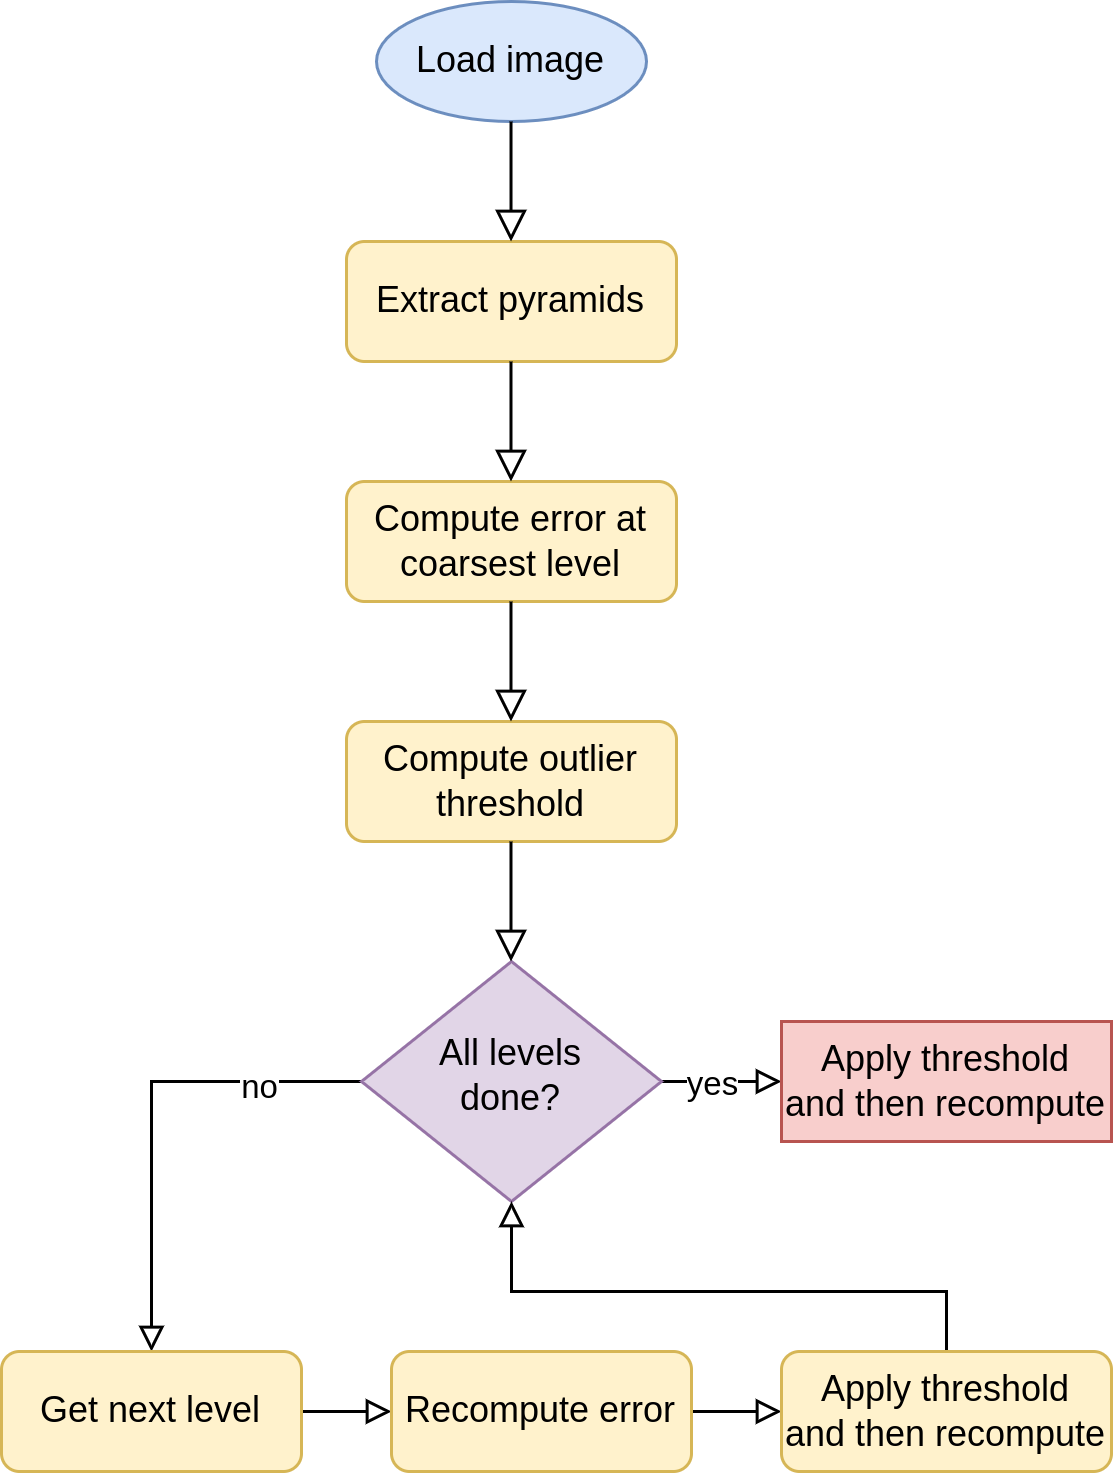
\includegraphics[width=.7\linewidth]{../assets/images/implementation-flow.png}
    \caption{Schema of the flow of implementation of the global motion estimation pipeline.}
    \label{fig:implementation-flow}
\end{figure}

\subsection{Block-Based Motion Estimation}
\label{sec:BBME}
The first piece of the architecture is the algorithm to compute the motion field to be used as ground truth.
In our case, we decided to implement a block matching motion estimation (BBME), as computing the motion field on blocks, rather than single pixels, can be much less computationally expensive.

The main idea of BBME is to divide the frame in blocks, and search for each block in the previous frame the corresponding block in the next frame.
This gives us the displacement of the block between the two frames, which is accounted as motion vector of the block.
This is the basic principle of BBME, from which derived a number of implementations that present differences mainly in two aspects:
\begin{enumerate}
    \item the size and shape of the block;
    \item the path that the searching procedure follows.
\end{enumerate}

During the project we implemented a number of these techniques:
\begin{itemize}
    \item exhaustive search;
    \item two-dimensional logarithmic search;
    \item new three-step search, from \cite{Li94};
    \item diamond search, from \cite{Zhu2000};
\end{itemize}

In the final implementation, the block matching method used is the one presented in \cite{Zhu2000}, known as diamond search (DS),  with a mean square error measure to compute (dis-)similarity between blocks.
Nonetheless, all the other methods are still present and by slightly changing the code they can be tested as well.

Here we briefly discuss the algorithm that we choose to implement and propose a small example for clarification.
The DS algorithm uses a peculiar diamond-shaped search pattern, which defines which positions will be used as target points where to center the block in the next frame to see if it corresponds to the block in the previous frame. In particular, the algorithm uses two slighlty different shapes depending on the current iteration (see \cref*{fig:ds-search-patterns}):
\begin{itemize}
    \item large diamond search pattern;
    \item small diamond search pattern.
\end{itemize}

\begin{figure}
    \centering
    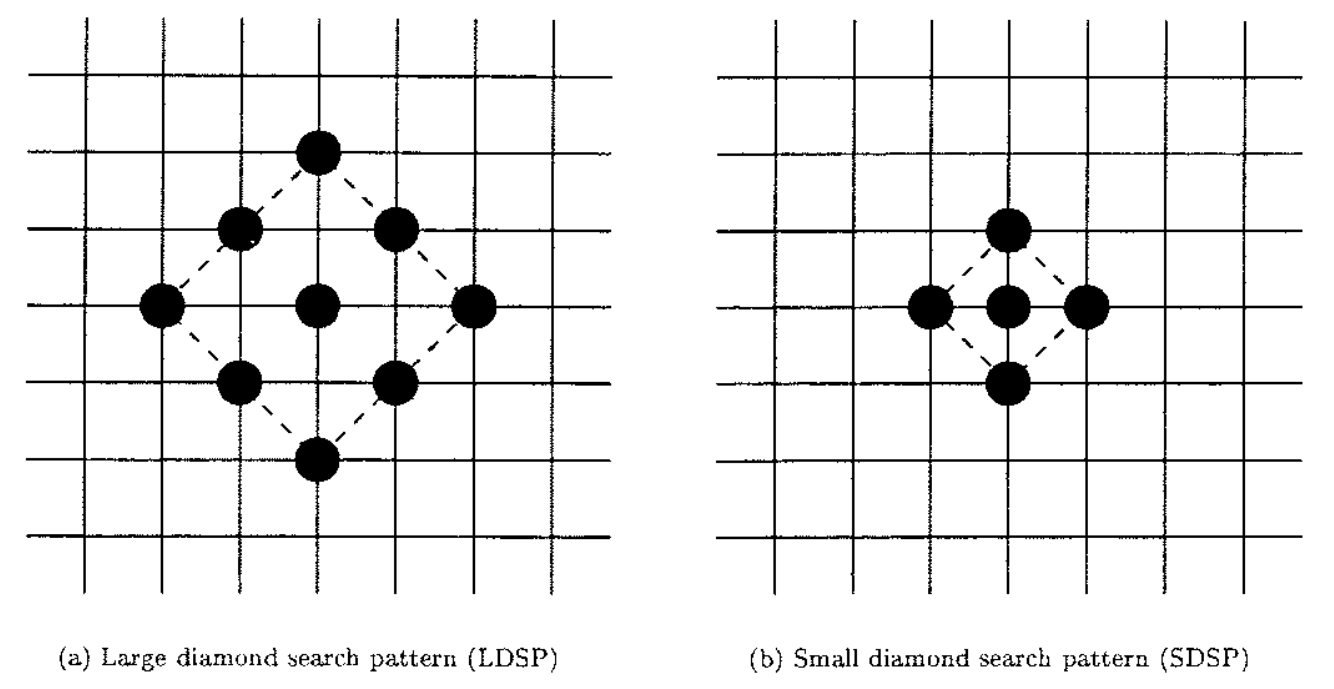
\includegraphics[width=.95\linewidth]{../assets/images/ds-search-patterns.png}
    \caption{Representation of the two DS algorithm search patterns}
    \label{fig:ds-search-patterns}
\end{figure}

The procedure is the following:
\begin{enumerate}
    \item the search starts with LDSP, meaning that we check the blocks centered in each one of the 9 positions; if the best match is the central position then we pass to the second step, otherwise we move to the best match position and re-use the LDSP;
    \item in the second step we use SDSP and look again for the best matching position among the 5 available, then return the best match position.
\end{enumerate}

\begin{figure}
    \centering
    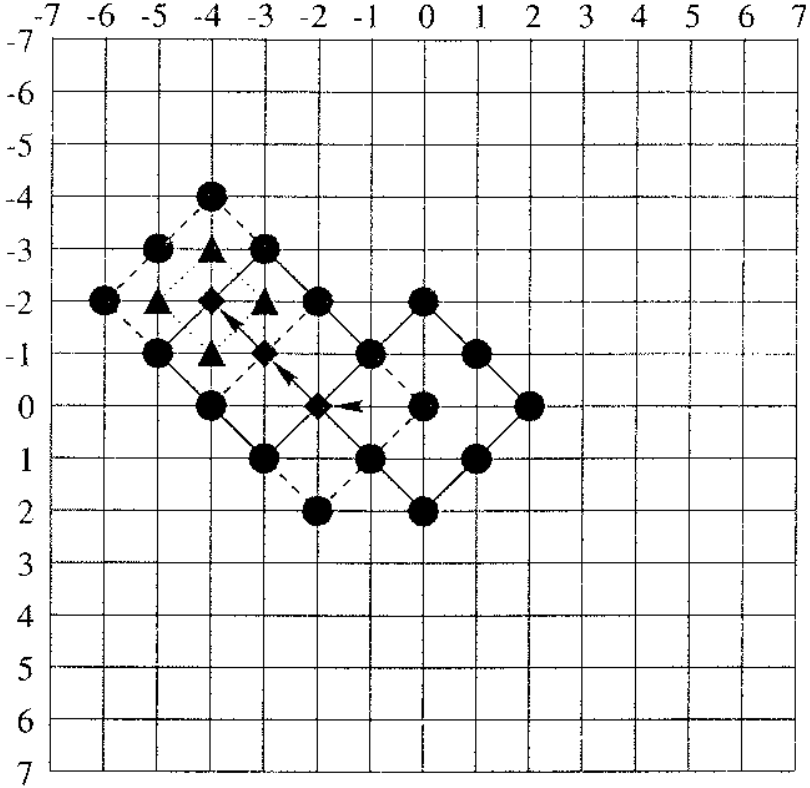
\includegraphics[width=.95\linewidth]{../assets/images/ds-exe.png}
    \caption{Example of run of diamond search algorithm for block matching motion estimation.}
    \label{fig:diamond-search-example}
\end{figure}

In \cref{fig:diamond-search-example} we can see an example of run. We can spot the three large-shape diamonds (the contour position are marked with circles) and the small shaped diamond (contour positions marked with triangles).
In this example the block matching algorithm started from $\{0,0\}$, then moved with the large diamond to $\{-2,0\}$, because this was the position that minimized the error between the block in the previous and the next frame. Then again with the large diamond the algorithm reached $\{-3,-1\}$ first, and $\{-4,-2\}$ after. Here the best matching position for the large diamond shape was $\{-4,-2\}$, therefore the algorithm stopped using the large diamond and started with the small diamond. Finally, the small diamond returned once again as best match position $\{-4,-2\}$, which was then returned as final matching position for the block in the previous frame.

\subsection{Affine Model Parameter Estimation}
\begin{figure*}[!h]
    \removelatexerror
    \begin{algorithm}[H]
    \DontPrintSemicolon
    
    \SetKwData{params}{\(a\)}
    \SetKwData{out}{outliers}
    \SetKwData{prevp}{prev\_pyrs}
    \SetKwData{curp}{cur\_pyrs}
    \SetKwData{prevf}{prev\_frame}
    \SetKwData{curf}{cur\_frame}
    \SetKwData{gt}{ground\_truth\_mfield}
    \SetKwData{est}{estimated\_mfield}
    
    \SetKwFunction{Pyr}{get\_pyr}
    \SetKwFunction{FirstEst}{first\_estimation}
    \SetKwFunction{Next}{next}
    \SetKwFunction{BM}{BBME}
    \SetKwFunction{Aff}{affine}
    \SetKwFunction{DetOut}{detect\_outliers}
    \SetKwFunction{Min}{minimize\_error}
    
    \KwIn{\textit{previous\_frame}, \textit{current\_frame}}
    \KwOut{\params \quad \texttt{//\(\;\)parameter vector}}
    \;        
    \prevp = \Pyr{previous\_frame}\;
    \curp = \Pyr{current\_frame}\;
    \params = \FirstEst{\prevp.\Next{}, \curp.\Next{}}\;
    \ForEach{\(l\) in levels}{
        \prevf = \prevp.\Next{}\;
        \curf = \curp.\Next{}\;
        \gt = \BM{\prevf, \curf}\;
        \est = \Aff{\params}\;
        \out = \DetOut{\gt, \est}\;
        \params = \Min{\prevf, \curf, \out}\;
        }
        
        \Return \params\;
        
        \caption{High-level pseudocode of our solution.}
        \label{alg:gme}
    \end{algorithm}


% prev_pyr = get_pyr(previous_frame)
% curr_pyr = get_pyr(current_frame)
% a = first_estimation(prev_pyr.pop(), curr_pyr.pop())
% for level in ([1,2]):
% 	curr = curr_pyr.pop()
% 	prev = prev_pyr.pop()
% 	ground_truth_mfield = BMME_motion_estimation(prev, curr)
% 	estimated_mfield = affine(a)
% 	outliers = detect_outliers(ground_truth_mfield, estimated_mfield)
% 	a = minimize_error(prev, curr, outliers)# update parameters
% return a
\end{figure*}
In \cref{sec:motion-models}, we presented the affine motion model, which is the one we decided to use in our implementation.

To get the motion vector of a certain position $p=\{x,y\}$ in the previous frame, we can solve the following formulation of the affine model:
\begin{equation}
    \label{eq:displacement-matrix-formulation}
    d(p, a) = A(p)\;a
\end{equation}
where $d(p, a)$ is the displacement for the position $p = \{x,y\}$, given the parameter vector $a$; $A[p]$ is an intermediate matrix that is computed as 
\begin{equation*}
    \label{eq:affine-model-parameter-matrix}
    A(p) = \begin{bmatrix}
        1 & x & y & 0 & 0 & 0 \\
        0 & 0 & 0 & 1 & x & y
    \end{bmatrix}
\end{equation*}

By encoding the estimation of the motion field in this way, the $p$-norm error we are trying to minimize (see \cref{eq:indirect-estimation}), gets rewritten in this way:

\begin{equation}
    \label{eq:pnorm-error}
    E = \sum_p{\left| d(p, a) - d(p) \right|^P}
\end{equation}
Here we introduce $d(p)$ as the ground truth motion vector (the one we get from the BBME as in \cref{sec:BBME}) and $P$ which specifies the grade of the $p$-norm used. In this case we decided to set $P=2$, following the procedure explained in \cite{WangBook}. Pay attention to the difference, in the formula, between $p$ (the position) and $P$ (the grade of the $p$-norm). 

The next step is to minimize the error in \cref{eq:pnorm-error} with respect to the parameter vector $a$.
The procedure in \cite{WangBook} states that we need to compute the gradient of $E$ w.r.t $p$, and then get the value of $a$ that sets the gradient to 0.

By using the matrix formulation explained in \cref{eq:displacement-matrix-formulation} and by setting the gradient $\nabla_a E = 0$, we obtain the following result:
\begin{equation}
    \label{eq:optimal-parameter-affine}
    a = \left (\sum_p A[p]^T A[p] \right )^{-1} \left (\sum_p A[p]^T d(x) \right)
\end{equation}

There are three interesting notes about \cref{eq:optimal-parameter-affine}:
\begin{enumerate}
    \item we are iterating over a set of positions $p$: it's interesting to notice that these points do not need to cover the complete scene, i.e. we can use only a subset of the image to optimize the parameters;
    \item each one of the points can be weighted with a weight $w(p)$ as shown in \cref{eq:optimal-parameter-affine-weighted};
    \item we can actually split the computation of the parameter vector $a = [a_1, a_2, a_3, b_1, b_2, b_3]$ in two different slices, $a_x = [a_1, a_2, a_3]$ and $a_y = [b_1, b_2, b_3]$, which can be computed in a specular way as shown in \cref{eq:optimal-parameter-affine-weighted-halved} this is useful to further reduce the complexity of the procedure.
\end{enumerate} 

\small
\begin{equation}
    \label{eq:optimal-parameter-affine-weighted}
    a = \left (\sum_p w(p) A[p]^T A[p] \right )^{-1} \left (\sum_p w(p) A[p]^T d(x) \right)
\end{equation}
\begin{equation}
    \footnotesize
    \label{eq:optimal-parameter-affine-weighted-halved}
    a_x = \left (\sum_p w(p) A_x[p]^T A_x[p] \right )^{-1} \left (\sum_p w(p) A_x[p]^T d_x(x) \right)
\end{equation}
where $A_x(p) = [1,x,y]$.

The form of the solution that we used in the implementation is the one reported in \cref{eq:optimal-parameter-affine-weighted-halved}.

\subsection{Hierarchical Robust Estimation}

The last part of the project is a strategy used to provide a robust estimation of the parameters for the affine motion model.
The proposed implementation is inspired by \cite{Dufeaux2000}, where the computation of the motion field takes place at different levels of resolution subsequently.

The main idea is to compute the parameter vector $a$ at a coarser resolution, and then use this coarser estimation to extract information useful for regularizing the estimation at finer resolutions. 
In practice, this translates in our code being structured as shown in \cref{fig:implementation-flow}: the two frames we use as previous and next frame are, first of all, transformed in multi-resolution pyramids, and then used iteratively for the process of parameter estimation.

Here we report a summary of the procedure used to implement the hierarchical robust etimation:
\begin{enumerate}
    \item for each iteration we get as input the frames at the corresponding level $l$ of the pyramid (at a finer resolution w.r.t the previous iteration at level $l-1$) and the parameter vector $a_{l-1}$ computed in the previous iteration;
    \item we use the (scaled) parameters $a_{l-1}$ to compute the error for each position $p$ in the frames at level $l$; error is computed as difference between the ground truth motion vector in $p$ and the motion vector obtained with the motion model in $p$ with parameters $a_{l-1}$;
    \item to detect the outliers we order all positions $p$ by the magnitude of the error, we set a fixed percentage \texttt{outlier\_percentage} and all the positions that fall in that percentage of higer-error-positions are marked as outliers;
    \item once we have marked all the outliers, we can proceed and compute the new estimate of the parameter vector $a_{l}$ ignoring the outliers;
    \item the new estimate will be returned to the next level $l+1$ of the hierarchical procedure, or simply returned to the caller of the function when we reach the last level.
\end{enumerate}
\section{Results}
\label{sec:04-results}

\subsection{Qualitative results}

To show the results of global motion estimation it is easier to use some qualitative information, also because the reader will understand it straightforwardly.

One of the applications that shows inuitively the implications of global motion estimation is camera motion compensation. 
Basically, if the video is recorded by a camera which is moving, we will see the two types of motion explained in \cref{sec:01-intro}: apparent and real. The aim of camera-motion compensation is to detect and remove the (apparent) motion which is caused only by the (ego)motion of the camera.

To show the results obtained we reported in image \red{qualitative-result-image} an example in which the reader can observe:
\begin{itemize}[noitemsep]
    \item first row position 1, the previous frame 
    \item first row position 2, the next frame 
    \item first row position 3, the compensated frame 
    \item second row position 1, the absolute difference between next and previous frame
    \item second row position 2, the motion field generated by the camera as it's returned by our estimation procedure
    \item second row position 2, the absolute difference between the next frame and the compensated one 
\end{itemize}

\red{image here}

\paragraph{How to interpret the results shown in \red{qualitative-result-image}} We should be able to notice in the results that the motion that we can register between the two frames is pretty large. In fact, we can see that a big part of the visual field seems to be moving in \red{ref second-row-position-1}.

But, if we compute the motion generated by the camera egomotion, we find out that the majority of the movement we record is apparent.
By estimating the motion generated by the camera, which is reported in  \red{ref second-row-position-2}, we can compensate the apparent motion in the previous frame.
When we compensate the previous frame we delete all the motion due to apparent motion and, therefore, if we compare the current frame and the compensated frame (see \red{ref second-row-position-3}) we are able to isolate real motion.

The results shown are consistent since the video from which the frames are taken was recorded with the camera moving in the horizontal direction while the person in the video was walking.

\subsection{Quantitative results}

To perform a numeric quantitative analysis of the results produced by the algorithm we used, once again, the compensation of the previous frame. Basically, in a video sequence where there is no real motion, but only camera motion, the compensation of the apparent motion should be enough tho make the current and the compensated frame identical.

Therefore, in \red{insert table}, we present some PSNR values for different video sequences. We annotated the table with some considerations about the videos, since PSNR value is influenced also about properties of the video like the strength of motion or the presence/absence of real motion.

\red{table here}
\section{Conclusions}
\label{sec:conclusions}

This project addresses the task of global motion estimation through the use of an indirect method for the estimation of apparent motion which is based on the affine motion model.

During the implementation of the tool, we built the following scripts:
\begin{itemize}
    \item \texttt{bbme.py} as Python module containing all the functions related to the various block matching motion estimation procedures that we have been trying;
    \item \texttt{motion.py} as Python module containing all the functions and constants needed in order to perform camera motion estimation and motion compensation;
    \item \texttt{results.py} as example of use of the packages modules to produce the results we used also to create this report.  
\end{itemize}

The approach we used proved to be efficient and robust, as long as the motion in the image is not too complex and as long as the background is not uniform and, therefore, the BBME algorithms are able to spot its motion.

The actual implementation is to be found in the following GitHub repository \url{https://github.com/Samaretas/global-motion-estimation}, where the reader can find all the commented scripts and try out the code.
In the repository it will be possible to run the basic example with \texttt{pan240.mp4}, whilst the other videos of the dataset can be found here \url{https://drive.google.com/drive/folders/1gZisWe4DEWpb_CoHkTi6OKnxhl5Ca_mT?usp=sharing}.

For more information on the code and how to perform a full-cycle execution of the pipeline, please refer to the Github repository.

This project presents some limitations that will be handled in future developments:
\begin{itemize}
    \item first, there is no automated way to set the distance between previous and next frame, in fact, often we need to set more than one frame of distance between \textit{previous} and \textit{next}, otherwise the motion is too small to compute GME;
    \item then, to have a comparison with other methods, like the ones cited before, we would need to insert this piece of code in a pipeline for video encoding, to record its performance both in accuracy and efficiency;
    \item finally, there are some intrinsic limitations to the task of GME, some of them are even presented in the results reported here, for instance the setting in which the scene is too noisy of the objects are bigger than the actual background.
\end{itemize}

\bibliography{bibliography.bib}{}
\bibliographystyle{IEEEtran}

\end{document}
